\def\year{2017}\relax
%File: formatting-instruction.tex
\documentclass[letterpaper]{article}
\usepackage{aaai17}
\usepackage{times}
\usepackage{helvet}
\usepackage{courier}
\usepackage{url} 
\usepackage{multicol}
\usepackage{array}
\usepackage{xcolor}
\usepackage{subcaption}

\usepackage{graphicx}
\graphicspath{ {images/} }

\usepackage[breaklinks=true]{hyperref}
\usepackage{breakcites}
\frenchspacing
\setlength{\pdfpagewidth}{8.5in}
\setlength{\pdfpageheight}{11in}
\pdfinfo{
/Title (Nasty, Brutish, and Short: What Makes Election News Popular on Twitter?)
/Author (Sophie Chou, Deb Roy) 
/Keywords (Twitter, News, Virality)}
\setcounter{secnumdepth}{0}  
 \begin{document}
% The file aaai.sty is the style file for AAAI Press 
% proceedings, working notes, and technical reports.
%
\title{Nasty, Brutish, and Short:\\
What Makes Election News Popular on Twitter?}
\author{Sophie Chou\\
MIT Media Lab\\
Cambridge, MA, USA\\
soph@media.mit.edu\\
\And
Deb Roy\\
MIT Media Lab\\
Cambridge, MA, USA\\
dkroy@media.mit.edu\\
}
\maketitle
\begin{abstract}
During the 2016 U.S. presidential elections, Twitter served as an important platform for the spread of news articles, which have significant influence on public opinion. Yet the sharing of stories is often based on innate emotional triggers, seldom rational. In our research, we seek to examine whether the emotional vocabulary of political news stories can lead to their popularity.To explore these questions, we construct a corpus of 2,650 news stories collected by scraping the websites of 13 different news organizations over 5 months. We then match these stories to all tweets that contain a link to them, resulting in 123,113 tweets by 20,964 Twitter users. Using the Harvard Inquirer lexicons, we automatically categorize the vocabulary in articles, coding stories for emotionality and positivity. We then run regressions between the independent variables of story length, emotionality, and positivity and the dependent variable of number of shares across 7 different political divisions of Twitter users, as well as the collective dataset. On the whole, we find Twitter users to favor stories that are Hobbesian in nature: nasty (negative in positivity), brutish (high in emotionality), and short (low in word count). However, differences emerge when considering different levels of political engagement among users.

\end{abstract}

 
\section{Introduction}
In the changing landscape of both journalism and politics, social media is playing an increasingly large role in mobilizing and spreading information to citizens. A Pew Research survey from August 2015 showed that nearly two-thirds of adults in the U.S. who are on Twitter use the platform to get news \cite{pew-Twitter-news}. All of these tweets lead to an impact on the outcome of political processes: since President Barack Obama's winning presidential bid in 2008, social media has been recognized as an important tool in political campaigning \cite{cogburn2011networked}. % MAKE IT STRONGER LINE ABOUT THE IMPACT OF SOCIAL MEDIA?
 
% In 2008, President Barack Obama's winning campaign was largely attributed to the success of his social media strategy, the first example of its kind. By establishing an online presence that recruited more than 3 million individual contributors and 5 million volunteers, Obama was able to create a grassroots political movement \cite{cogburn2011networked}. Publicity and public sound bites matter-- especially when it’s free and has the potential to go viral.
  
The popularity of sharing articles on social media also marks an important shift in the role of the news consumer from armchair reader to information propagator. Whereas news used to be broadcast to the reader, each reader now has the powerful potential to broadcast stories to his or her own audience. Yet previous work, including Berger and Milkman's study on what makes the New York Times' ``most emailed list'' and Hansen et. al.'s research on sentiment and news-sharing, show that the impulse to share content is often predictably emotional in nature \cite{berger2012makes, hansen2011good}. In short, the desire to share a certain story is often universally impulsive, regardless of context. In the case of political news, this impulse can have a large impact on reach of political messages -- an impact that is not always equally distributed. 

 \subsection{Hypotheses}
% With the important role of social media in politics and the often emotionally charged nature of content-sharing in mind, 
We ask the following question in our research: 

\begin{itemize}
\item Does the emotional vocabulary of political news stories have an impact on its Twitter popularity that persists beyond political affiliation?  
\end{itemize}

To test this question, we focus on three key aspects of stories: length, emotionality, and positivity. We choose these three aspects based on behavioral theories of the internet and studies of political news, detailed in the section below. We hypothesize the following behavior in our dataset of stories and tweets:

\begin{itemize} 
    \item \textbf{H1:} Story length has a \emph{negative} correlation with Twitter shares, due to the effects of the internet attention economy and overexposure to political media \cite{goldhaber1997attention}.
    \item \textbf{H2:} Emotionality has a \emph{positive} correlation with Twitter shares, consistent for viral content in general \cite{berger2012makes}.
    \item \textbf{H3:} Positivity has a \emph{negative} correlation with Twitter shares, due to the nature of political news \cite{berger2012makes, hansen2011good}.

\end{itemize}

For each of these three independent variables (story length, emotionality, positivity) we repeat analyses across three views of the data: first, the entire dataset; then, by political candidate followed amongst users who follow only one candidate; and finally, by the number of political candidates followed (degree of political engagement), to look for differences amongst different populations of political tweeters.

\section{Literature Review}  

For several decades, there has been an assumption that the kind of emotion a story evokes has a significant impact on the likelihood for it to be well-received. Yet defining that connection, and quantifying the type of emotion that matters, remains to be explored.

In Galtung and Ruge's seminal work on news values, negativity is proposed as a positive attribute for news stories. In other words, ``bad news is more newsworthy than good news'' \cite{galtung1965structure}. However, more recently, Berger and Milkman's study found that positive content was more likely to make the New York Times most-emailed list than negative content \cite{berger2012makes}. The results of Hansen et. al’s research, which focuses on Twitter, counters that finding, showing that negativity is a boon in news stories’ popularity -- yet positivity is more likely to lead retweets overall \cite{hansen2011good}.

Political news, however, is a unique category of news, and this past election -- where one-in-four Americans report disliking the presidential candidates -- appears to have a negative overtone \cite{dislike-candidates}. In a study of responses to the 2012 election campaign on Twitter, it was found that for both candidates, the majority of tweets were far more negative in tone than positive \cite{mitchell2013twitter}.
    
To compare the sharing of election news stories on Twitter versus patterns of general virality in the news, we calculate the negativity of stories, and how that relates to popularity. We also examine the effects of the degree of combined emotionality in the content. In Berger and Milkman's study, both highly positive and highly negative content were more likely to become viral than stories of low emotional valence, and we expect the same to hold for political news \cite{berger2012makes}. 

Finally, the abundance of information on the web has created new challenges and questions about the kind of content being processed by readers. This paradox -- between the ease of accessibility to information and the increasingly limited bandwidth of consumers -- is described as one of the challenges of being in an attention economy \cite{goldhaber1997attention}. High-impact events like the presidential elections intensify this effect -- about 60 \% of Americans reported feeling exhausted by media coverage of the elections in July of 2016 (Gottfried 2016). To explore the effects of the attention economy on the reading of political news, we examine story length and how it relates to sharing popularity.
 
\section{Data Collection} 

\subsection{News Dataset}
For our news dataset, we scraped articles from the RSS feeds of news publications every hour over five months and 13 publications: CNN, Fox News, the New York Times, The Wall Street Journal, The Washington Post, The Los Angeles Times, The Associated Press, Reuters, McClatchy, Politico, Buzzfeed, The Huffington Post, and NPR.

To create a diverse set of election stories, we include sources that have mostly conservative audiences or mostly liberal audiences (based on a 2014 survey); come from mixed primary media formats (television, paper, online, radio); are viewed as ``legacy'' (over a hundred years old) or ``new'' media (founded online within the last 10 years); focus solely on political news (Politico, McClatchy); and are newswire services (the Associated Press, Reuters news) \cite{PoliticalPolarization}. 
  
We look at stories from January 1, 2016 (the start of the election year) to May 1, 2016. This time period captures the bulk of the primary election, when coverage of multiple presidential candidate contenders creates greater variety in news stories for our analysis.

Articles are processed in a 3-step pipeline. After collecting the links to the full content of the news stories from each publication's RSS feed, we pass each link to a structured content parser that extracts entities and features from the raw HTML. The story text is then passed into a binary MaxEnt classifier for election news. The classifier, which was built for prior research, uses Bag-of-word features, is trained on a balanced dataset of 1,000 manually labeled news articles, and performs with a F-score of 0.90 \cite{vijayaraghavan-thesis}. 

\subsection{Tweets Dataset}
We start with the firehose of all tweets between January 1, 2016 and May 1, 2016 in our data process. Tweets pass through a similiar pipeline as news stories. First, we sort all tweets with an election classifier which has been shown to be able to detect election-related tweets with an F-score of 92\% \cite{vvr_electome2016}. We then filter by those that share a link (which might potentially be a news story). 

We collect and sort a total of 16,667,685 tweets as election-related and containing at least one URL in the text, an average of 4,000,000 per month and 140,000 per day.

\subsection{Combined Dataset}
The final step of our data collection process is to extract, expand and connect the links shared in our election-related tweets with articles in our database.
 
Twitter automatically formats all links into a shortened ``t.co'' format, so we first expand all links in tweets (16.6 million), then use regular expressions to see if the final destination of the expanded link matches a query-truncated URL of a story in our database. We checked the validity of 382 billion url-story matches in less than a day by running the processes on the Amazon Web Services cloud computing platform in parallel using the Gnu-parallel command line tool \cite{tange2011gnu}.

In total, we found that 30\% of the election stories we tracked were shared on Twitter during the time period of January 1st through May 1st. There were 137,986 tweets that contained a link to 6,911 unique stories (out of 22,960). Since we chose the story to be the unit of analysis in this thesis, we then eliminated any stories that were shared by less than 10 tweets. This left a total of 2,650 distinct articles shared in 123,113 tweets by 20,956 Twitter users.

\subsubsection{Descriptive Findings}
Story sharing behavior follows an approximate power law distribution. On average, stories are shared 46 times.

\begin{figure}[t!]
\centering 
  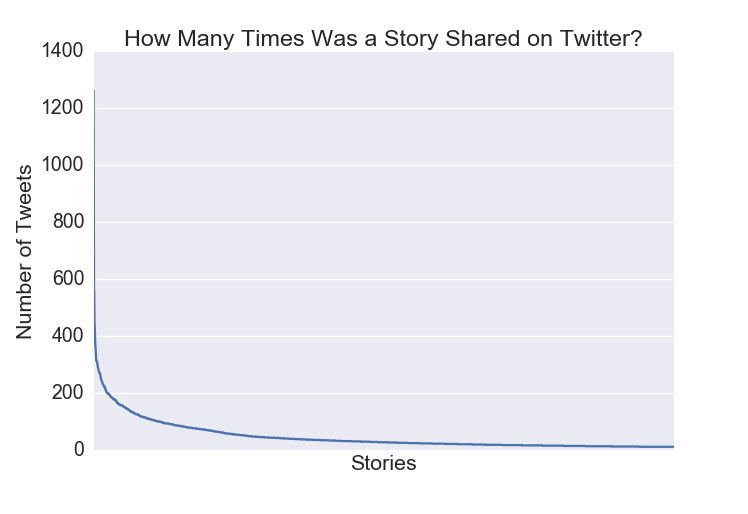
\includegraphics[width=0.8\columnwidth]{story-share-dist}   
  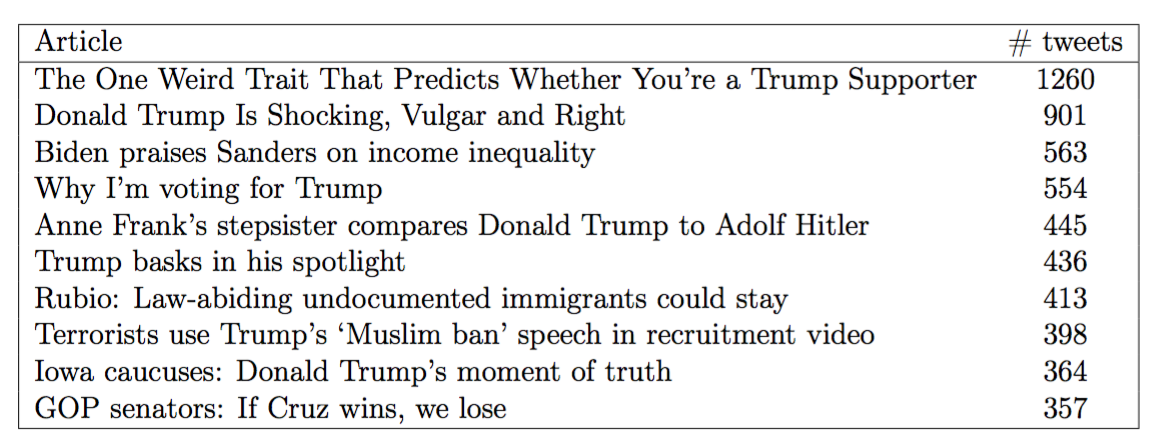
\includegraphics[width=0.8\columnwidth]{top-10-stories} 
  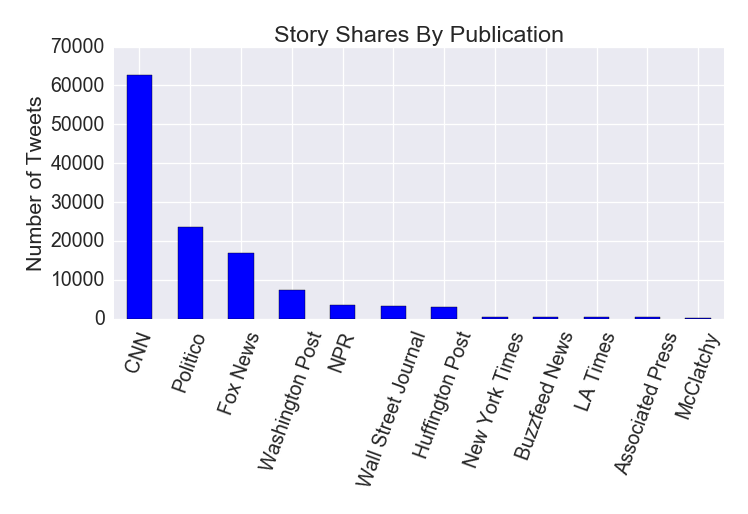
\includegraphics[width=0.8\columnwidth]{all-stories-by-pub} 
  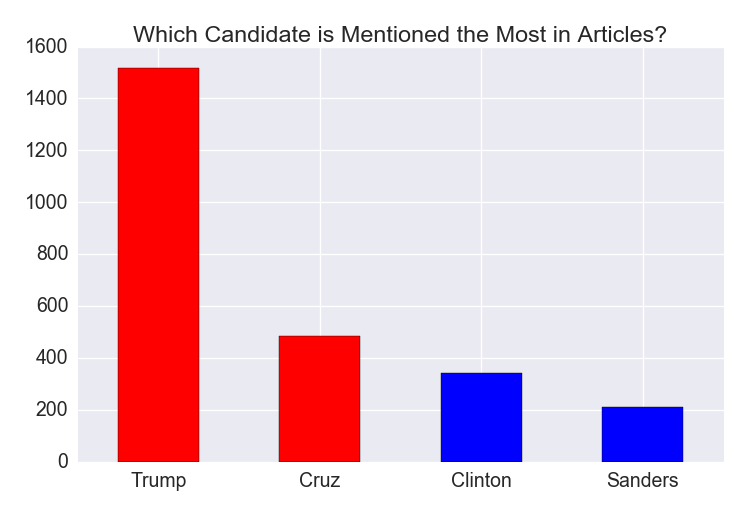
\includegraphics[width=0.8\columnwidth]{candidate-mentions}  
  \caption{Number of story shares by publication
    \label{fig:shares-by-pub}}
\end{figure} 

% \begin{figure}[t!]
% \centering 
%   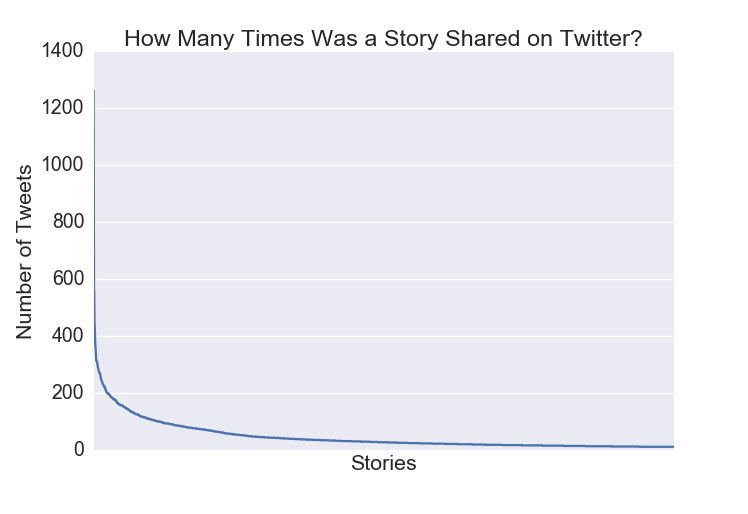
\includegraphics[width=0.8\columnwidth]{story-share-dist}  
%   \caption{Distribution of Story Shares
%     \label{fig:story-share-dist}}
% \end{figure} 


% \begin{figure}[t!]  
% \centering 
%   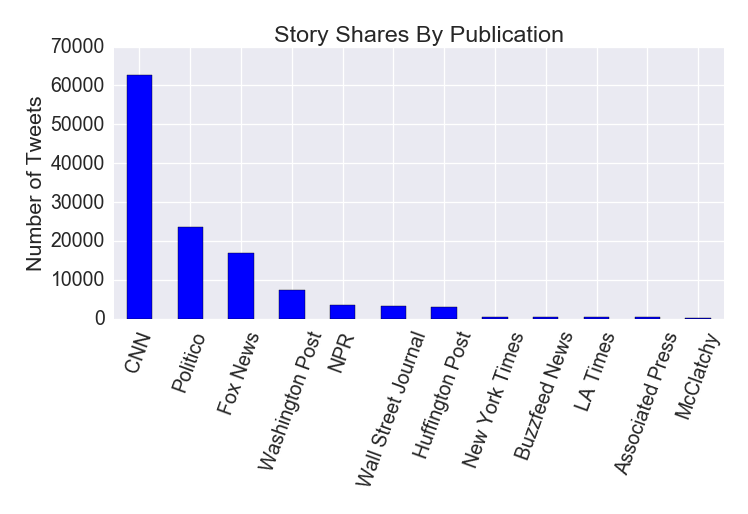
\includegraphics[width=0.8\columnwidth]{all-stories-by-pub}  
%   \caption{Number of story shares by publication
%     \label{fig:shares-by-pub}}
% \end{figure} 


CNN, Politico, and Fox have the highest number of stories shared by tweets in our dataset. This is likely due to the volume of and focus on political content for these outlets (figure \ref{fig:shares-by-pub}).  
% Because our data pipeline detailed in the previous section looks for election-related news, outlets which focus on political news are more likely to show up in our results.
%\newpage %force table to get on the next page

% \begin{figure}[t!]  
% \centering 
%   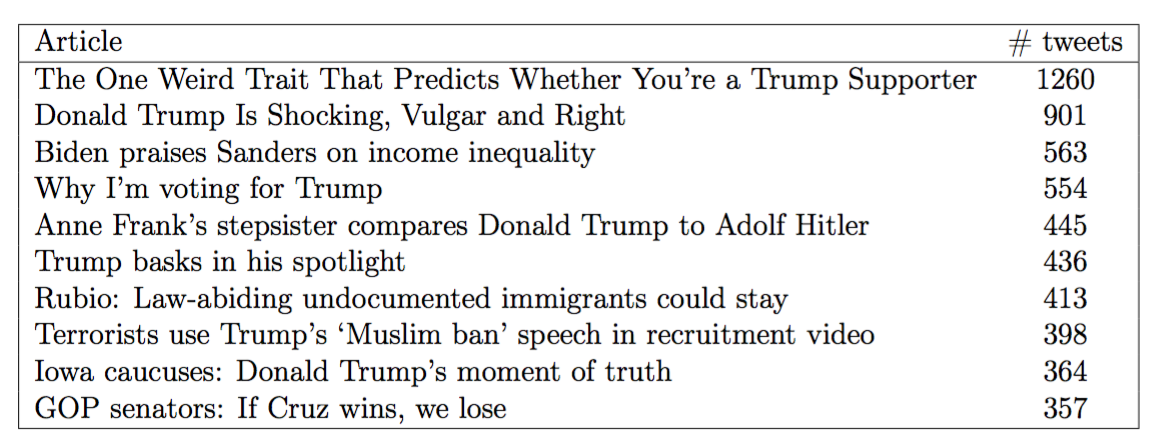
\includegraphics[width=0.8\columnwidth]{top-10-stories}  
%   \caption{Top 10 Most Shared Articles
%     \label{fig:top-10-stories}}
% \end{figure} 

% \begin{figure}[t!]  
% \centering 
%   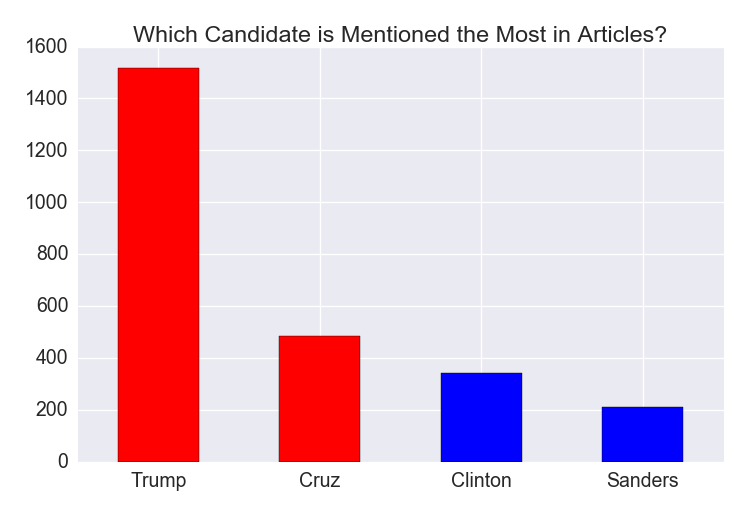
\includegraphics[width=0.8\columnwidth]{candidate-mentions}  
%   \caption{Most frequently mentioned candidate in stories
%     \label{fig:most-freq-candid}}
% \end{figure} 


Examining the top 10 most shared stories, Donald Trump is by far the most ``tweetable'' candidate, dominating the list with 7 out of 10 stories featuring his name in the title. Coding each story by the most frequently mentioned candidate mentioned in the body of the text, Trump has nearly three times as much coverage at nearly 60\% as the runner-ups, Ted Cruz and Hillary Clinton. The large number of stories with Cruz as the most-mentioned candidate are likely due to his association to Trump as a Republican runner-up: 96\% of stories where Cruz is the most-mentioned candidate feature Trump as the second-most frequently occuring. 

\section{Measuring Political and Emotional Engagement}

\subsection{Emotional Coding}
For the emotional coding of news articles, we use dictionaries from the Harvard General Inquirer, a lexicon that is popular for computerized content analysis \cite{stone1963computer}. In Berger and Milkman's study of online virality, automated coding using the LIWC system showed results that were significantly positively correlated with the output of manual coding \cite{berger2012makes}. The Inquirer is a public-use alternative to the LIWC system. 

In particular, we use the \emph{Positiv} and \emph{Negativ} collections, a set of 1,915 well-established words signifying positive outlook (not including words for \emph{yes}) and 2,291 words signifying negative outlook (not including words for \emph{no}), respectively. Repeating the same metrics from Berger and Milkman's study, we calculate emotionality as $\frac{count(positiv \mid negativ)}{count(words)}$ and positivity as $\frac{count(positiv)}{count(words)} - \frac{count(negativ)}{count(words)}$.

% Repeating the same metrics from Berger and Milkman's study, we calculate positivity as the
%difference between the percentage of words from the \emph{Positiv} and \emph{Negativ} collections in an article, and emotionality as the percentage of words that were classified from either collection. 

 \subsection{Followership as a Proxy for Political Engagement}
Previous studies find that users on Twitter tend to show network homophily within political groups, or that ``like follows like''. In addition, followership of only Democratic or only Republican official accounts can be used as a reasonable estimator of party loyalty. Those accounts that follow only the officials of one party tend to demonstrate more closeness with other users in their political party than those who do not \cite{colleoni2014echo}. Due to the highly individualized nature of the 2016 elections, candidate loyalty did not necessarily imply goodwill towards the party. As a result, look specifically at what candidates users follow. 

For general levels of political engagement, we look at the number of political candidates a Twitter user follows as a proxy for how likely they are to share political news. For single-candidate Tweeters, we divide users by the candidate they follow. At the time of data collection completion (May 1, 2016), the top two candidates by delegate count in each party were Hillary Clinton (D), Bernie Sanders (D) and Donald Trump (R) and Ted Cruz (R), so we split users into these four groups. 

% \begin{figure}[t]
%     \centering
%     \begin{subfigure}{0.8\linewidth}
%         \centering
%         %\includegraphics[width=\textwidth, trim={12mm 6mm 24mm 10mm}, clip]{daily_activity_old}
%         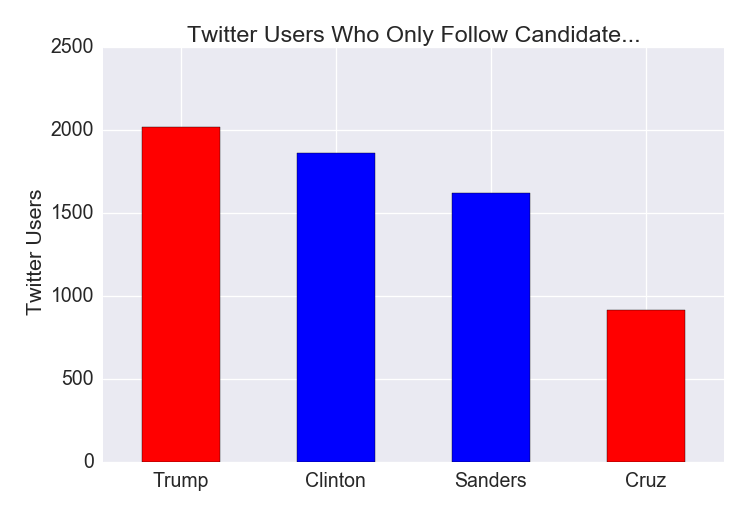
\includegraphics[width=\textwidth]{users-by-candid} 
%     \end{subfigure}
%     ~
%     \begin{subfigure}{0.8\linewidth}
%         \centering
%         %\includegraphics[width=\textwidth, trim={3mm 0mm 2mm 2mm}, clip]{weekly_activity}
%         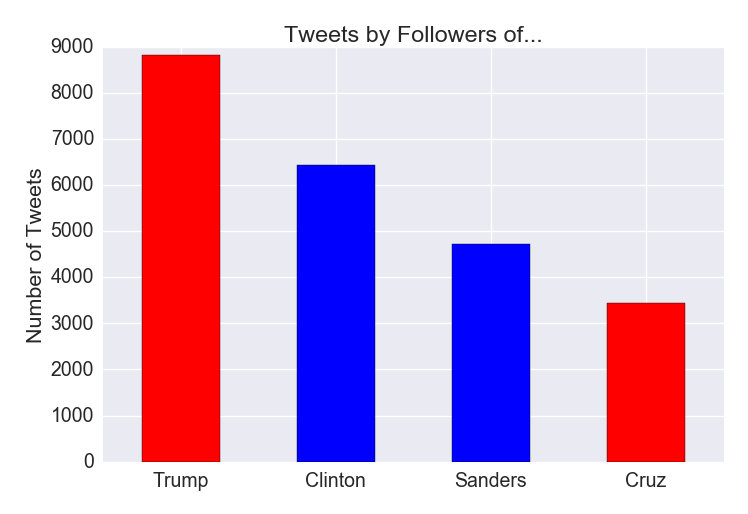
\includegraphics[width=\textwidth]{tweets-by-candid}  
%     \end{subfigure}
%     \caption{Daily (A) and weekly (B) activity patterns on Yak Yak (green) and Twitter (blue).}    
%     \label{fig:temporal-activity-patterns}
% \end{figure}


\begin{figure}[t!]  
\centering 
  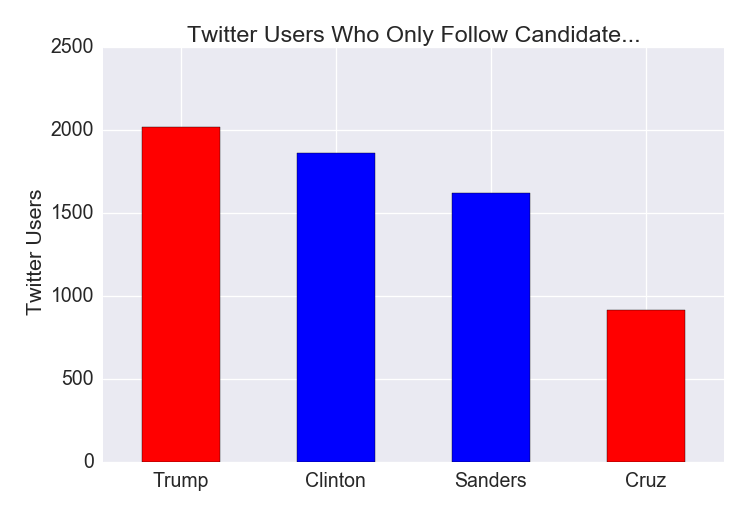
\includegraphics[width=0.8\columnwidth]{users-by-candid}  
%   \caption{Number of Tweets by Each Segment
%     \label{fig:users-by-candid}}
% \end{figure} 

% \begin{figure}[t!]  
% \centering 
  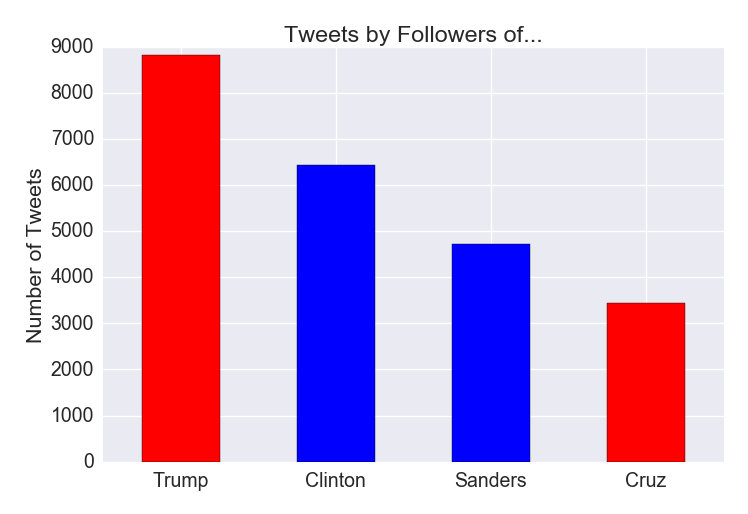
\includegraphics[width=0.8\columnwidth]{tweets-by-candid}  
  \caption{Number of tweets by candidate group
    \label{fig:tweets-by-candid}}
\end{figure} 

\subsubsection{Candidate Followership}
Our dataset contains 6,406 unique single-candidate Twitter users. Trump-only followers lead with about 31\%, followed closely by Clinton-only (29\%), then Sanders (25\%) and Cruz (14\%). 37\% of tweets sharing articles come from Trump-only followers versus 27\% for Clinton-only, 20\% for Sanders-only, and 14.6\% for Cruz. We also observe the nature of the content being shared by each group. Again, across all four segments, Republican candidate Trump leads the top number of mentions in stories shared (see figure \ref{fig:who-shares-stories-about}).


% \begin{figure}[t]
%     \centering
%     \begin{subfigure}{0.5\linewidth}
%         \centering
%         %\includegraphics[width=\textwidth, trim={12mm 3mm 10mm 2mm}, clip]{comments-per-port-dist}
%         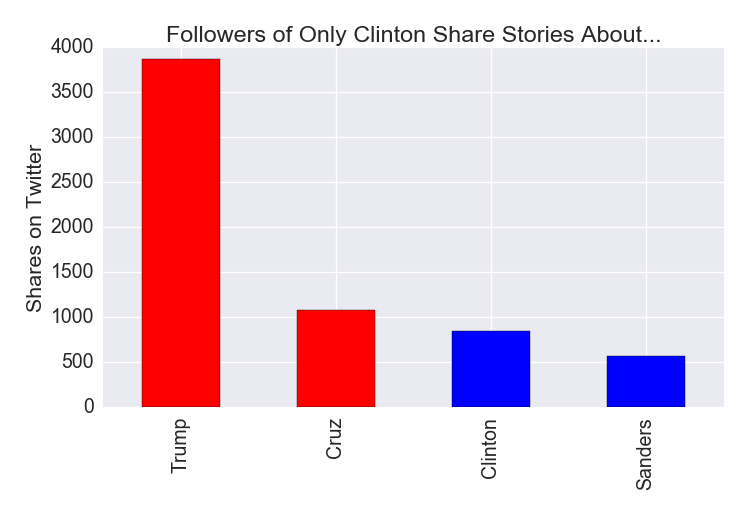
\includegraphics[width=\textwidth]{clinton-camp-shares}
%     \end{subfigure}%
%     ~
%     \begin{subfigure}{0.5\linewidth}
%         \centering
%         %\includegraphics[width=\textwidth, trim={3mm 4mm 15mm 13mm}, clip]{yy-post-rating-dist}
%         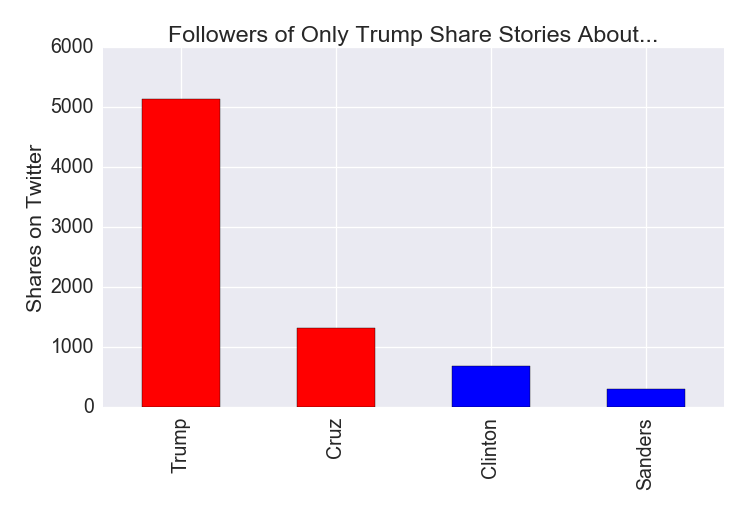
\includegraphics[width=\textwidth]{trump-camp-shares}  
%     \end{subfigure}
%     ~
%     \begin{subfigure}{0.5\linewidth}
%         \centering
%         %\includegraphics[width=\textwidth, trim={3mm 4mm 15mm 13mm}, clip]{figures/yy-comments-rating-dist}
%         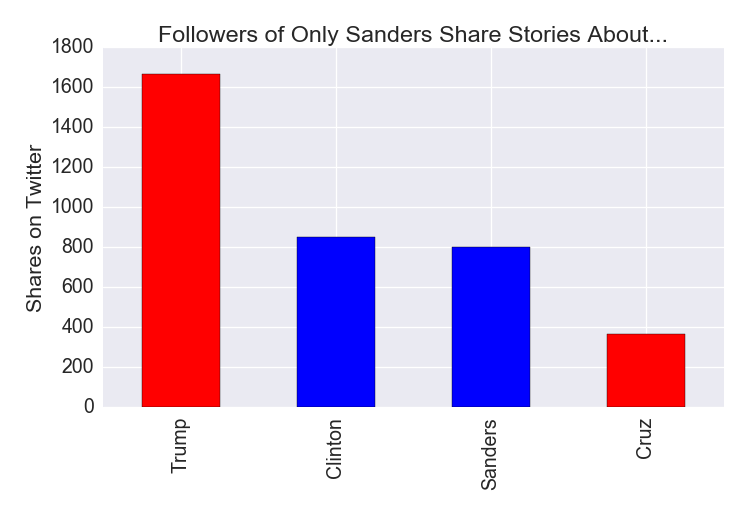
\includegraphics[width=\textwidth]{sanders-camp-shares}  
%     \end{subfigure}%
%      ~
%     \begin{subfigure}{0.5\linewidth}
%         \centering
%         %\includegraphics[width=\textwidth, trim={3mm 4mm 15mm 13mm}, clip]{figures/yy-comments-rating-dist}
%         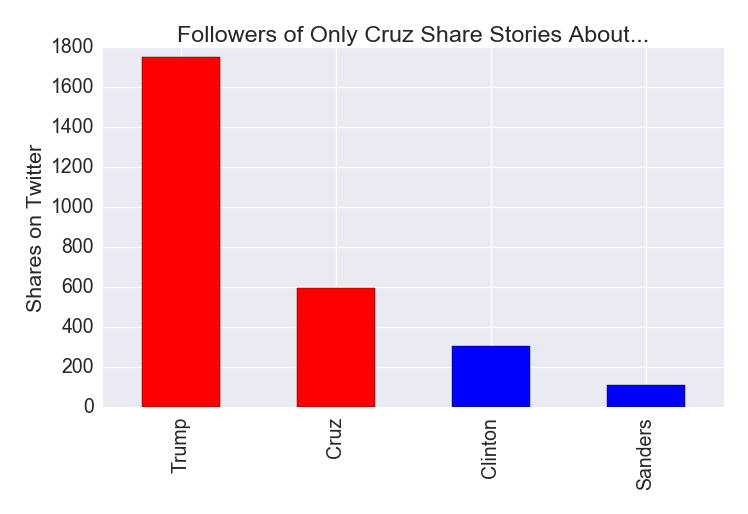
\includegraphics[width=\textwidth]{cruz-camp-shares}  
%     \end{subfigure}%
%     \caption{Yik Yak. (A) Distribution of number of replies per post. (B) Distribution of ratings (number of upvotes/down-votes) of posts. (C) Distribution of ratings of post replies.}
%     \label{fig:yy-dist-replies-ratings}
% \end{figure}

%% Most popular mentioned candidate by ea. camp
% \begin{figure}[htbp!] 
% \centering 
%  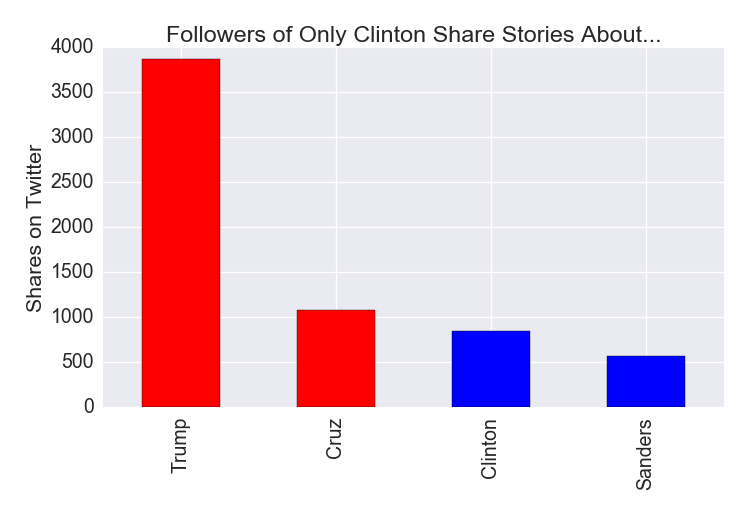
\includegraphics[width=0.8\columnwidth]{clinton-camp-shares}
%  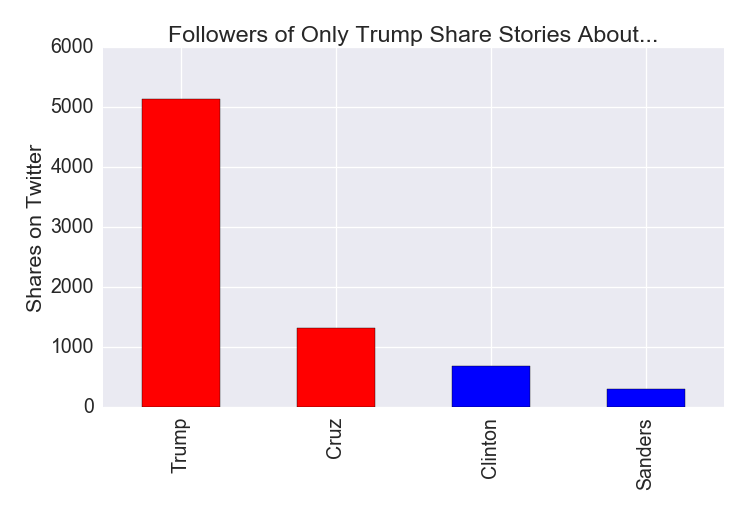
\includegraphics[width=0.8\columnwidth]{trump-camp-shares}  
%  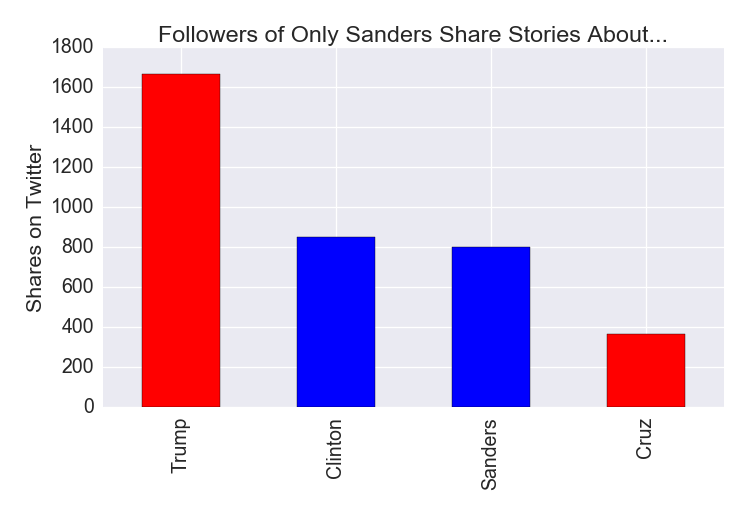
\includegraphics[width=0.8\columnwidth]{sanders-camp-shares}  
%  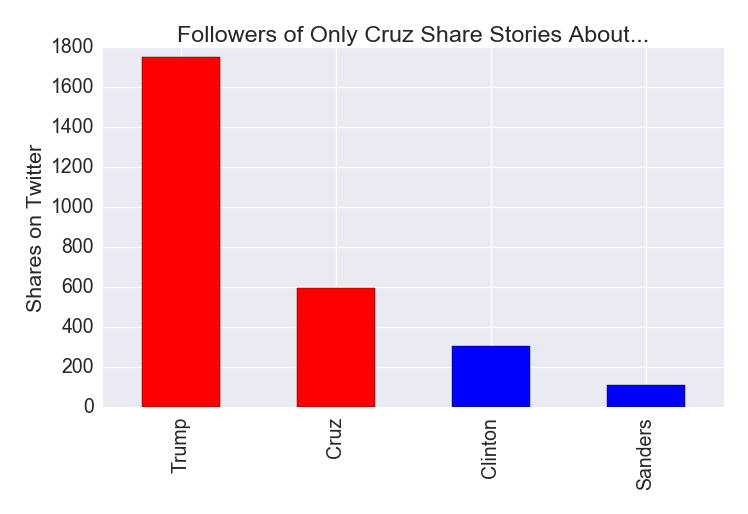
\includegraphics[width=0.8\columnwidth]{cruz-camp-shares}  
%   %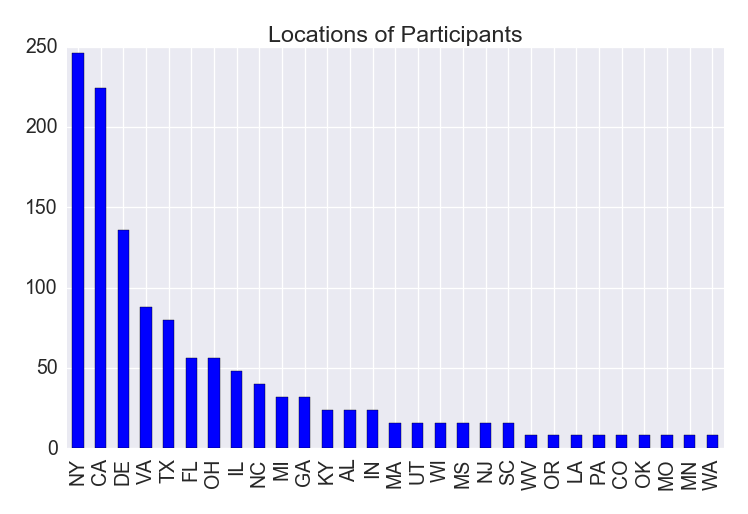
\includegraphics[width=0.32\columnwidth]{location_study2} 
%   \caption{Most frequently mentioned candidate in stories, by group
%     \label{fig:users-tweets-by-candid}}
% \end{figure}

\begin{figure}[htbp!] 
\centering 
 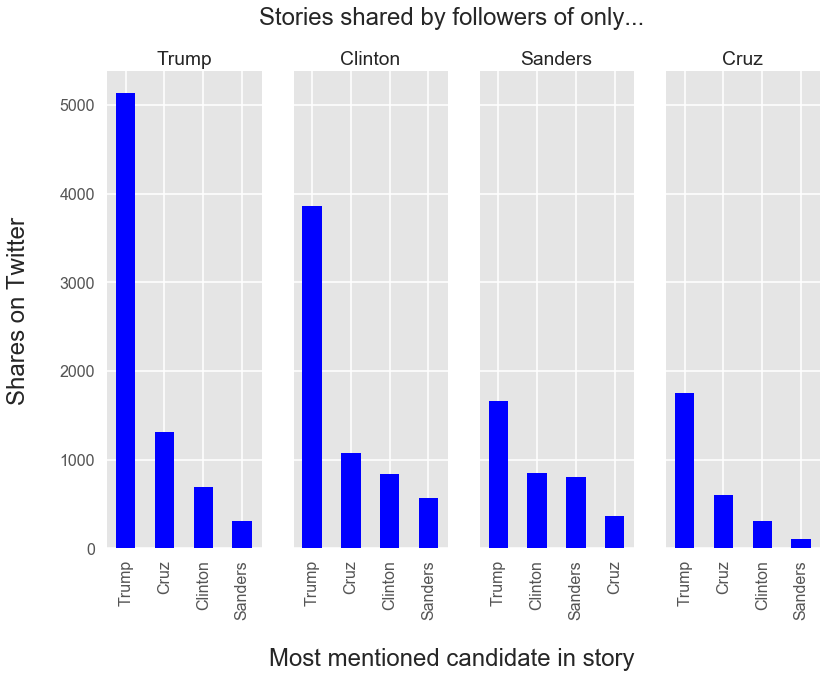
\includegraphics[width=1.0\columnwidth]{who-shares-stories-about}  
  \caption{Most frequently mentioned candidate in stories, by group
    \label{fig:who-shares-stories-about}}
\end{figure}
 
\subsection{Political Engagement}

% Descriptives of candididate 0/1/3+:
% * Bar chart of \% by \# Following
% * Number of tweets by each camp
% * Most popular orgs by each camp
% * Most popular story by each camp
% * Most mentioned candid in each camp

\begin{figure}[t!]  
\centering 
  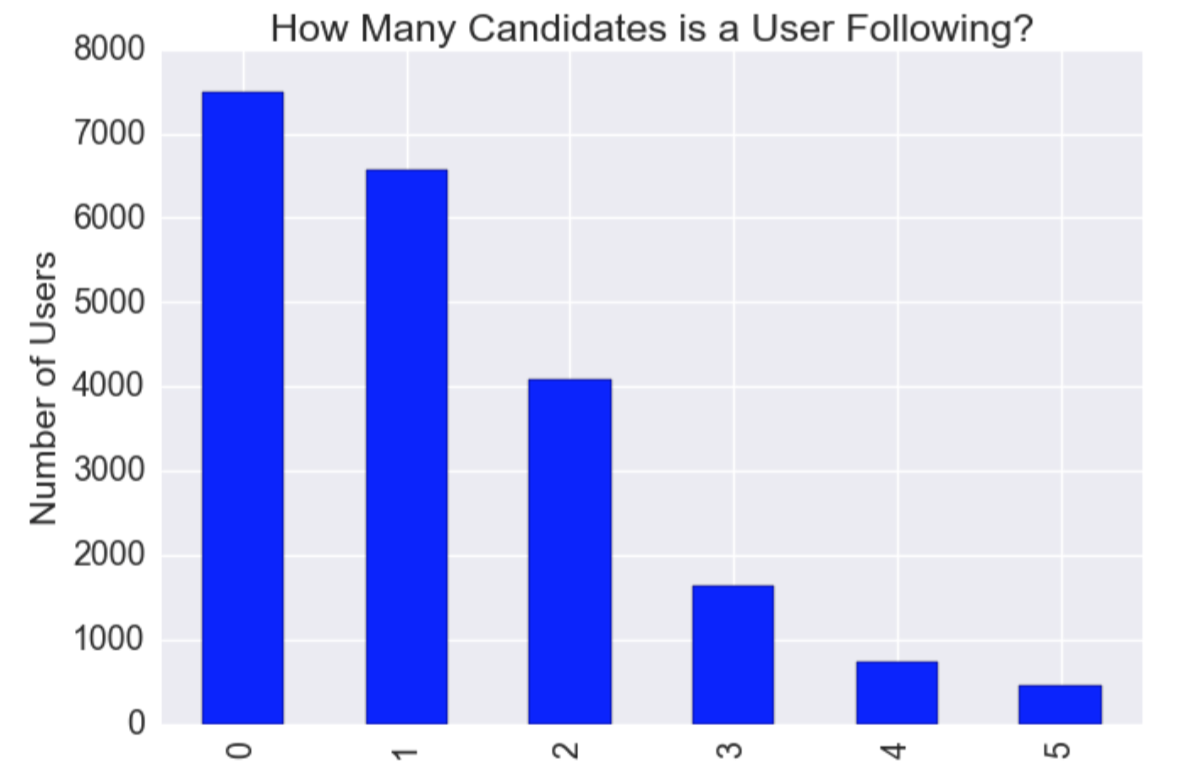
\includegraphics[width=0.8\columnwidth]{users-vs-engagement}  
%   \caption{Number of users by level of political engagement
%     \label{fig:users-vs-engagement}}
% \end{figure}


% \begin{figure}[t!]  
% \centering 
  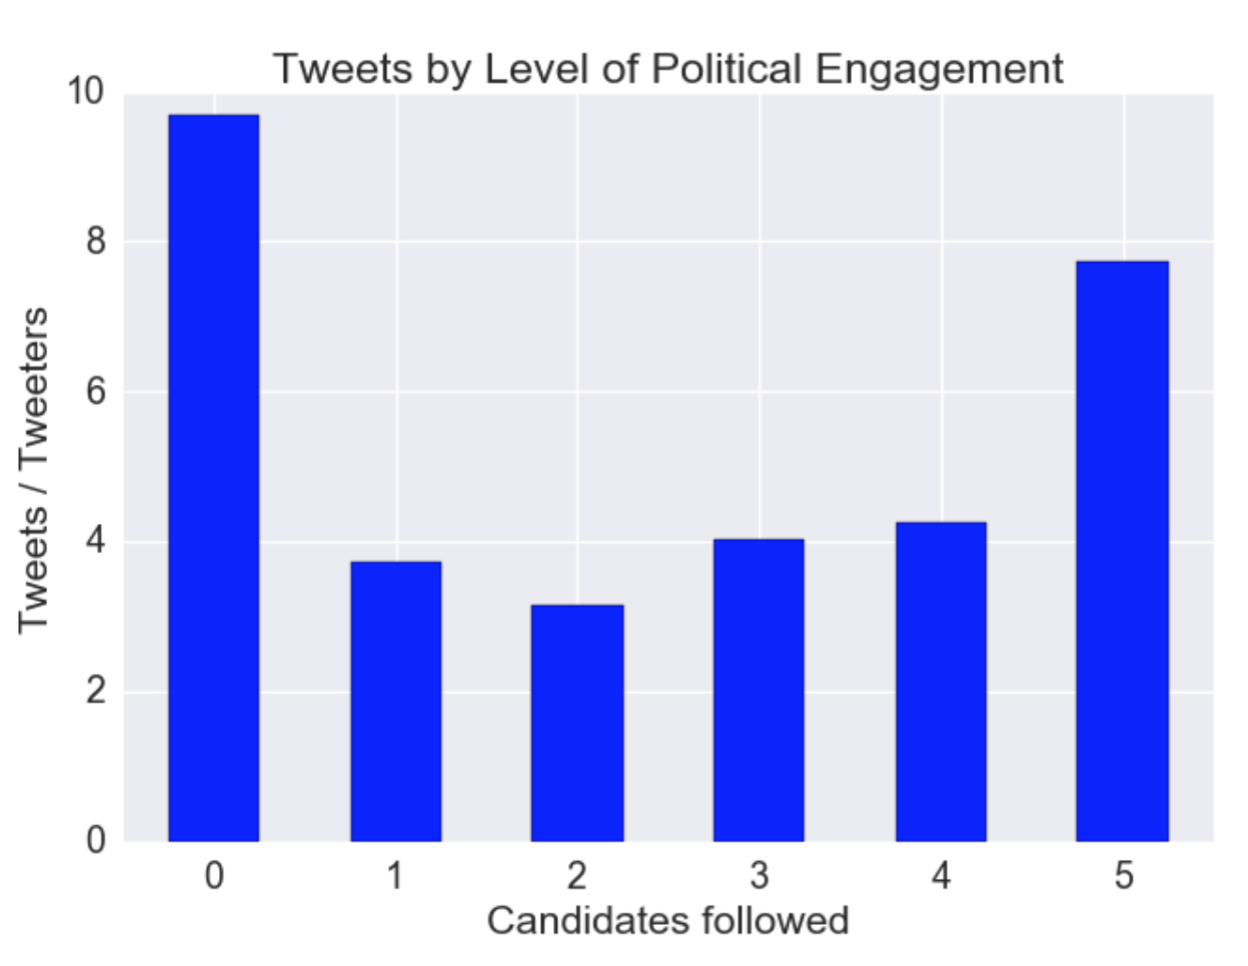
\includegraphics[width=0.8\columnwidth]{tweet-ratio-vs-engagement}  
  \caption{Tweets per user by level of political engagement
    \label{fig:tweet-ratio-engagement}}
\end{figure}

36\% of Twitter users in our dataset follow none of the four political candidates, followed by 31\% who follow one candidate, 20\% who follow two, and 13\% who follow three or more candidates. We see a negative curvlinear relationship between the number of candidates followed (level of observed political engagement) and the ratio of political news tweets per user (figure \ref{fig:tweet-ratio-engagement}).


In the following analyses, we segment levels of political engagement into three groups for the sake of comparison:

\begin{itemize}
  \item \textbf{the unaffiliated} (those who follow no presidential candidates, but do tweet about political news)
  \item \textbf{the loyal} (those who follow one and only one presidential candidate, and tweet about political news)
  \item \textbf{the political aficionados} (those who follow all 4 (or more) candidates, and tweet about political news).
\end{itemize}


\section{Analysis} 
For each of these three independent variables (story length, emotionality, positivity) we repeat analyses across three views of the data: first, the entire dataset; then, by political candidate followed amongst users who follow only one candidate; and finally, by the number of political candidates followed (degree of political engagement), to look for differences amongst different populations of political tweeters.


\subsection{Methodology}

Since our dependent variable, tweet volume, is a set of discrete counts that are positively truncated, we use negative binomial regression models for our analysis \cite{scott1997regression}. The distribution of tweet volume is not a normal distribution, and it is not recommended to perform a log transformation on count data to fit it to an OLS regression unless there is little dispersion in the data \cite{o2010not}. Poisson models are a subset of negative binomial models without the dispersion parameter. In our analyses, we see that the negative binomial model provides the best fit and that our data is overdispersed, as the dispersion parameter $\theta$ is greater than 1.   

In addition, we apply a log transformation on the independent variable of story length, as its distribution follows an approximate power law. Both emotionality and positivity are more normally distributed so we do not transform the data.
In each case, we compare our findings to those using linear and Poisson regression models, and are able to achieve the same significant results. 

\subsection{All Data}

% Table created by stargazer v.5.2 by Marek Hlavac, Harvard University. E-mail: hlavac at fas.harvard.edu
% Date and time: Thu, Dec 22, 2016 - 11:14:33
\begin{table}[!htbp] \centering 
  \caption{Story Popularity vs. Story Traits, All Tweets} 
  \label{} 
\begin{tabular}{@{\extracolsep{5pt}}lc} 
\\[-1.8ex]\hline 
\hline \\[-1.8ex] 
 & \multicolumn{1}{c}{\textit{Dependent variable:}} \\ 
\cline{2-2} 
\\[-1.8ex] & num\_tweets \\ 
\hline \\[-1.8ex] 
 log(story length) & $-$0.088$^{***}$ \\ 
  & (0.017) \\ 
  & \\ 
 emotionality & 6.279$^{***}$ \\ 
  & (1.770) \\ 
  & \\ 
 positivity & $-$5.978$^{***}$ \\ 
  & (2.013) \\ 
  & \\ 
 constant & 4.296$^{***}$ \\ 
  & (0.117) \\ 
  & \\ 
\hline \\[-1.8ex] 
Observations & 2,650 \\ 
Log Likelihood & $-$12,761.660 \\ 
$\theta$ & 1.361$^{***}$  (0.035) \\ 
Akaike Inf. Crit. & 25,531.320 \\ 
\hline 
\hline \\[-1.8ex] 
\textit{Note:}  & \multicolumn{1}{r}{$^{*}$p$<$0.1; $^{**}$p$<$0.05; $^{***}$p$<$0.01} \\ 
\end{tabular} 
\end{table} 



\subsubsection{Story Length}
Overall, we find a consistently negative correlation of high significance between story length and Twitter volume ($\beta=-0.088$, $p<0.01$). 
This aligns with our hypothesis \textbf{H1:} that shorter stories are more likely to be shared, due to competing resources in the attention economy.
 
\subsubsection{Emotionality}
Overall, we find a consistently positive correlation of high significance between emotionality and Twitter volume ($\beta=6.279$, $p<0.01$). This confirms \textbf{H2:} that emotionality has a \emph{positive} correlation with Twitter shares, consistent for viral content in general \cite{berger2012makes}.

\subsubsection{Positivity}
Overall, we find a consistently negative correlation of high significance between positivity and Twitter volume ($\beta=−5.978$, $p<0.01$). This finding supports \textbf{H3:} Positivity has a \emph{negative} correlation with Twitter shares, due to the nature of political news and contrary to generalized findings \cite{berger2012makes, hansen2011good}.

\subsection{By Degree of Political Engagement}
For the three levels of political engagement (the unaffiliated, single-candidate followers, and political aficionados) we repeat the same methods and variables in determining our correlations. Again, we test all three models (OLS, Poisson, and NB) for consistency and report the results of the negative binomial model. Overall, we find that: 

The unaffiliated show the same patterns as the general dataset with a negative correlation between story length and Twitter shares ($\beta=-0.283$, $p<0.01$), positive correlation between emotionality and Twitter shares ($\beta=10.718$, $p<0.01$), and a negative correlation between positivity and Twitter shares ($\beta=-4.968$, $p<0.05$).

The loyal, on the other hand, show a slight positive correlation between story length and number of Twitter shares ($\beta=0.156$, $p<0.01$). For emotionality ($\beta=5.577$, $p<0.01$) and positivity ($\beta=-7.754$, $p<0.01$), the trends remain the same. We hypothesize that if following a single candidate can serve as a proxy for candidate loyalty, then perhaps the correlation signifies a willingness to read and share more complex content on behalf of the candidate and a deeper degree of political involvement.

We see the same effects for the political aficionado group, again, a small but significant positive correlation between story length and number of tweets ($\beta=0.205$, $p<0.01$). For this group, we found no significant correlations between emotionality and Twitter popularity, although there was a significant negative correlation (as before) between positivity and tweets ($\beta=-6.043$, $p<0.05$). Again, this suggests a potential difference in levels of engagement with political news. 

\subsection{By Candidate} 

We divide Twitter users into four segments: Trump-only, Clinton-only, Sanders-only, and Cruz-only followers and repeat the same regressions within each population. 

Overall, we were unable to find a significant difference in the direction of correlations in any of the three independent variables between these candidate groups and single-candidate followers (the loyal) at large. However, we did find differences in magnitudes of the coefficients; most notably a strong negative correlation between postivity and number of tweets for Trump-only followers, about two and a half times in magnitude ($\beta=-14.684$, $p<0.01$) of the rest of tweeters ($\beta=−5.978$, $p<0.01$). 

As discussed in the section above, all single-candidate followers that showed a significant correlation between story length and number of Twitter shares showed a slight positive correlation.

\section{Conclusion}

For the general population of election tweeters, we find that:
\begin{itemize}
    \item Shorter stories are more likely to be shared on Twitter (\textbf{H1})
    \item Stories high in emotional words, both negative and positive, are more likely to be shared on Twitter (\textbf{H2})
    \item Stories that are less positive are more likely to be shared on Twitter (\textbf{H3})
\end{itemize}

These results are aligned with our expectations of the limitations of the attention economy, the emotional nature of content virality, and the idea that ``bad news is more newsworthy than good news'', confirming Galtung and Ruge's classical theory, along with Hansen et. al.'s more recent work \cite{galtung1965structure,hansen2011good}.

However, there are small but significant differences in the number of political candidates a user followed and the length of the stories that were likely to be shared. Although the unaffiliated (and the general population of tweeters) tend to prefer short stories, both the loyal and political aficionados prefer longer stories. This suggests a deeper level of engagement with political content versus the general population, which might have a more impulsive mechanism for sharing articles, leaving room for future research.

\section{Limitations and Future Work}  
The 2016 elections were an unusual time period for both traditional and social media. Twitter users on all sides of the political spectrum focused on Donald Trump, which may have limited findings. Futhermore, our dataset was limited to a small but diverse set of publications. Potential ways to create a more complete dataset include: Expanding the set of publications tracked, using machine learning methods to match tweets with stories, applying a more nuanced analysis of the story text, and including additional signals in the Twitter user data, such as the inferred political leaning of the person and the interaction between that leaning and the content shared. Still, our analysis provides a first view of article sharing on Twitter in a unique and eventful election year with large responses on social media.

\bibliography{nasty-brutish-short-poster}
\bibliographystyle{aaai} 
 
\end{document}
